% Report for the SE.LLMA candidate assignment. Built from RESEARCH_NOTE.md, with the method written out.
% Build (run twice, from this folder):  pdflatex report.tex
\documentclass[11pt,a4paper]{article}
\usepackage[T1]{fontenc}
\usepackage[utf8]{inputenc}
\usepackage[sc]{mathpazo}
\usepackage{tgpagella}
\linespread{1.06}
\usepackage{microtype}
\usepackage[margin=2.6cm]{geometry}
\usepackage{amsmath,amssymb}
\usepackage{booktabs,array}
\usepackage{graphicx}
\usepackage{xcolor}
\usepackage{enumitem}
\usepackage[font=small,labelfont=bf]{caption}
\usepackage{titlesec}
\usepackage{parskip}
\definecolor{accent}{HTML}{1D4ED8}
\usepackage[colorlinks=true,linkcolor=black,urlcolor=accent]{hyperref}
\graphicspath{{../results/}}

\titleformat{\section}{\Large\bfseries}{\thesection}{0.6em}{}
\titleformat{\subsection}{\large\bfseries}{\thesubsection}{0.6em}{}
\titlespacing*{\section}{0pt}{1.6em}{0.5em}
\titlespacing*{\subsection}{0pt}{1.1em}{0.3em}
\setlist{itemsep=0.35em,topsep=0.4em}
\DeclareMathOperator{\IPR}{IPR}
\DeclareMathOperator{\med}{med}
\DeclareMathOperator{\MAD}{MAD}
\newcommand{\norm}[1]{\lVert #1 \rVert}

\begin{document}

% ------------------------------------------------------------------ cover page
\begin{titlepage}
\thispagestyle{empty}
\vspace*{3.2cm}
{\color{accent}\rule{2.4cm}{2.5pt}}\par
\vspace{1.0cm}
{\fontsize{27}{33}\selectfont\bfseries Can a published weight edit be found from the weights alone?\par}
\vspace{0.9cm}
{\Large A test of weight-only edit detection on Qwen3.5-0.8B\par}
\vspace{2.6cm}
{\large Research report\par}
\vspace{0.25cm}
{\large SE.LLMA candidate assignment on \emph{Sparks of Weight-Space Programming}\par}
\vfill
{\large Francis Tembo\par}
\vspace{0.25cm}
{\large November 2026\par}
\vspace{1.0cm}
{\small Code, results and notebook: \url{https://github.com/FrancisTembo/weight-space-programming}\par}
\end{titlepage}

% ------------------------------------------------------------------ body
This report is the longer version of \texttt{RESEARCH\_NOTE.md}, with the method written out.
The numbers from my experiment are documented in \texttt{results/}, and the companion notebook is
\texttt{notebooks/weight\_edit\_detection.ipynb}. The figures in section~1 come from the logs the
article's authors released. The article is \emph{Sparks of Weight-Space Programming},
\url{https://rikiyat.github.io/blog/weight-space-programming/}.

\section{Critical read of the article}

\subsection{Strongest evidence}

The most convincing results are the tiny-network ones that use no model feedback, such as writing a
game-playing network in one reply. I did not check those. I did check that the published
Qwen3.5-0.8B edit rebuilds from its patch to the exact released weights.

\subsection{Apparent limitations}

The article's ``50 forward passes'' were a long feedback loop. The run took 158 turns and 20.3
hours. One pass ran up to hundreds of practice problems on the original and edited model and
returned the accuracy difference, which climbed from $+6$ to $+40$ points. This is optimisation
through repeated feedback, not reading weights and knowing the answer.

\subsection{What the article does and does not justify}

I think the article justifies this much: a frontier model with feedback might be able to find a
small edit that fixes one particular failure. It does not show that this is better than standard
methods, because it ran no baseline with steering or fine-tuning. It also does not show that it
brings new capabilities.

\section{Question and hypothesis}

\subsection{The question}

If someone publishes weights containing a malicious or restrictive edit, can it be found from the
weights alone, without a fingerprint or the original model weights?

\subsection{Why it matters for Swedish models}

From my understanding, SE.LLMA builds on third-party open model weights. If weight inspection
catches such edits, it is a cheap safeguard. If not, every adopted checkpoint needs behavioural
checks in Swedish.

\subsection{Two claims and how they are judged}

I tested two claims, and fixed the rules for judging them before the held-out run.

\begin{center}
\small
\begin{tabular}{@{}l >{\raggedright\arraybackslash}p{0.39\textwidth} >{\raggedright\arraybackslash}p{0.36\textwidth}@{}}
\toprule
 & \textbf{A. Screening: is there an edit?} & \textbf{B. Localisation: where, given a suspect layer?} \\
\midrule
Rule & A layer alarms if its statistic exceeds the highest among six clean development layers. & The detector names 64 neurons \\
\addlinespace
Supported & Recall $\ge 0.80$, at most 1 false alarm on 18 other clean layers & Mean precision $\ge 0.80$ \\
\addlinespace
Challenged & Recall $< 0.50$, or more than 1 false alarm & Mean precision $< 0.50$ \\
\bottomrule
\end{tabular}
\end{center}

I had expected claim A to fail, because exploration had revealed two pristine layers scoring above
the published edit. I also threw out a previous, more favourable estimate, because it used the true
edited neurons to choose what to score.

\section{Experiment}

\subsection{The edit}

In each layer the model's MLP computes
\[
  y = W\,\bigl(\sigma(W_{\mathrm{gate}}\,x) \odot W_{\mathrm{up}}\,x\bigr),
\]
where $W \in \mathbb{R}^{d \times n}$ is the output matrix, with $d = 1024$ and $n = 3584$, and
$\sigma$ is the SiLU activation. Column $w_j$ of $W$ and row $j$ of $W_{\mathrm{gate}}$ and of
$W_{\mathrm{up}}$ belong to neuron $j$.

An edit of the published kind changes 64 columns of $W$. Each changed column loses a multiple $m$
of its component along one unit direction $u$:
\[
  w_j' = w_j - m\,u\,(u^\top w_j), \qquad j \in S, \quad |S| = 64 .
\]
For the whole matrix the change is $\Delta W = -m\,u\,c^\top$, where $c_j = u^\top w_j$ for
$j \in S$ and $c_j = 0$ otherwise. It has rank one and touches only the columns in $S$. After the
edit, the component of a changed column along $u$ is $(1 - m)\,u^\top w_j$. I measure the size of
an edit as
\[
  \rho = \frac{\norm{\Delta W}_F}{\norm{W}_F} .
\]

For the published edit I measured $m = 6.00$ in both layers, with more than 99.99\% of the squared
norm of the change in a single direction. Its size is $\rho = 0.106$ in layer~15 and
$\rho = 0.081$ in layer~19.

A synthetic edit is built the same way. The direction $u$ is either one of the top 8 left singular
vectors of a random sample of 1{,}024 columns of $W$, which is a direction the layer already uses,
or a random unit vector. $S$ is the 64 columns with the largest $|u^\top w_j|$, and $m$ is set so
that $\rho$ is 0.03, 0.05 or 0.09.

\subsection{The spectral detector}

Write the singular value decomposition of a layer's output matrix as
$W = \sum_k \sigma_k\, a_k v_k^\top$ with $\sigma_1 \ge \sigma_2 \ge \dots$\,. A change confined to
a few neurons appears as a singular vector of that matrix that sits on those neurons: the term
$-m\,u\,c^\top$ has a right vector supported on $S$, and when it is large enough beside the
singular values of the clean matrix, one of the leading right singular vectors of the edited
matrix sits mostly on $S$.

To measure how concentrated a unit vector $v$ is, I use its inverse participation ratio,
\[
  \IPR(v) = \sum_{j=1}^{n} v_j^{4} .
\]
It equals $1/n$ when $v$ is spread evenly over all $n$ neurons and $1/q$ when it is spread evenly
over $q$ of them. The statistic of a layer is
\[
  T = n \max_{k \le 16} \IPR(v_k) ,
\]
so $T = 1$ for an evenly spread vector and $T = n/64 = 56$ for one spread evenly over 64 neurons.
The detector names the 64 neurons with the largest $|v_{k^\ast j}|$, where $k^\ast$ is the index
that gives the maximum, and it reports $a_{k^\ast}$ as the direction of the edit.

\subsection{The balance detector}

This is the alternative method. It uses the fact that a neuron's output weight norm normally
tracks its input norms. For each neuron let
$o_j = \log \norm{w_j}$, $g_j = \log \norm{W_{\mathrm{gate}}[j,:]}$ and
$p_j = \log \norm{W_{\mathrm{up}}[j,:]}$. I fit
\[
  o_j = \alpha\, g_j + \beta\, p_j + \gamma + r_j
\]
by least squares in three rounds, where each round after the first leaves out the 5\% of neurons
with the largest $|r_j|$ from the round before. The residuals are then scaled robustly,
\[
  z_j = \frac{r_j - \med(r)}{1.4826\,\MAD(r) + 10^{-12}} ,
  \qquad \MAD(r) = \med\bigl(|r - \med(r)|\bigr) ,
\]
where the small constant keeps the denominator from being zero. The statistic of the layer is
the mean of the 64 largest $|z_j|$. The detector names those 64
neurons.

\subsection{Decision rules}

Let $D$ be the six clean development layers. The alarm threshold of a detector is
$\tau = \max_{\ell \in D} T_\ell$, and a layer alarms when its statistic is greater than $\tau$.
Recall is the share of the 28 held-out edits at $\rho = 0.09$ whose layer alarms. False alarms are
counted on the 18 clean layers outside $D$. If $N$ is the set of 64 neurons a detector names, its
precision is $|N \cap S| / 64$. For the spectral detector I also report the cosine
$|a_{k^\ast}^\top u|$ between the recovered direction and the true one.

\subsection{Held-out test and controls}

The held-out test is 84 new synthetic edits of the published kind, with new seeds, at 3\%, 5\% and
9\% of the layer's weight norm. They sit in seven layers where no edit had been tried before,
although I had already seen the clean statistics of every layer. I judge the claims at 9\%. The
published edit is 8.1\% and 10.6\%.

The controls are the unedited model (for false alarms), three random edits of the same size on the
published edit's neurons, and the alternative detector under the same rules. Prompting and decoding
controls do not apply, because the detectors never run the model.

\subsection{Swedish measurement}

For the Swedish measurement I use next-token loss on 84 held-out Swedish passages (UD Talbanken)
and 32 English questions (GSM8K). For a passage with tokens $x_1, \dots, x_t$ the loss is
\[
  \mathcal{L} = -\frac{1}{t-1} \sum_{i=2}^{t} \log p(x_i \mid x_1, \dots, x_{i-1}) ,
\]
in nats per token. I report the mean over passages of
$\mathcal{L}_{\mathrm{edited}} - \mathcal{L}_{\mathrm{base}}$, with a 95\% interval from 2{,}000
bootstrap resamples of whole documents.

\section{Results}

\begin{center}
\small
\begin{tabular}{@{}lcc@{}}
\toprule
At 9\% edit size, 28 held-out edits & Spectral & Balance \\
\midrule
A. Recall at the threshold & 0.00 & 0.11 \\
A. False alarms on 18 clean layers & 0 & 1 \\
\textbf{A. Verdict} & \textbf{challenged} & \textbf{challenged} \\
\addlinespace
B. Mean precision at 64 & 0.77 & 0.18 \\
\textbf{B. Verdict} & \textbf{inconclusive} & \textbf{challenged} \\
\addlinespace
Median rank of the edited layer, of 24 & 4 & 18 \\
Mean precision at 5\% and 3\% edit size & 0.11, 0.07 & 0.02, 0.01 \\
\bottomrule
\end{tabular}
\end{center}

\begin{figure}[h]
\centering
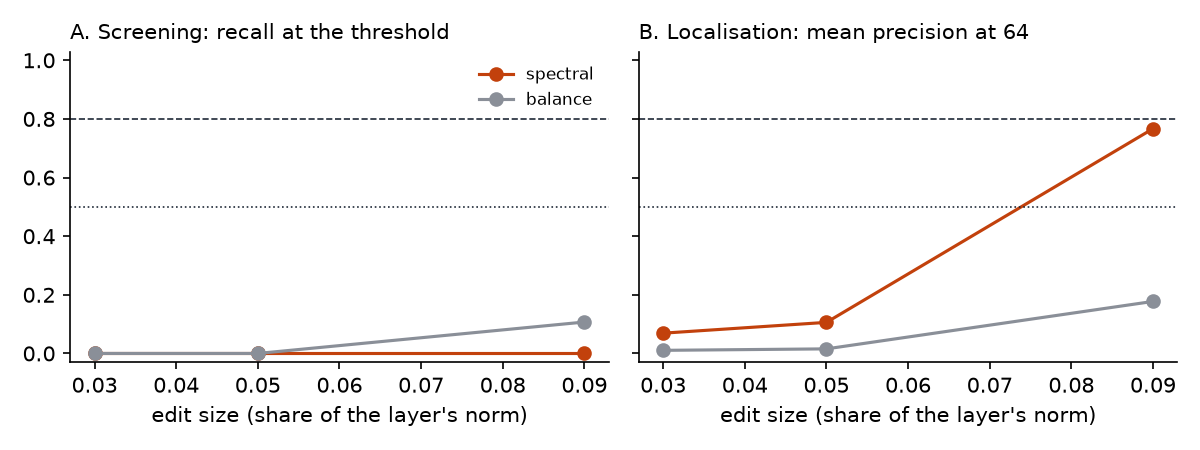
\includegraphics[width=0.92\textwidth]{fig_sweep.png}
\caption{Recall at the threshold (left) and mean precision at 64 (right) against edit size, for
the 84 held-out synthetic edits. The dashed and dotted lines mark the 0.80 and 0.50 bands.}
\end{figure}

\begin{itemize}
\item On the published edit (seen in exploration, reproduced here), the spectral detector names 59
of the 64 edited neurons in each layer and recovers the direction (cosine 0.94 and 0.95). Even so,
the two layers rank 4th and 3rd of 24 and do not alarm, and the two layers above them are untouched
(Figure~\ref{fig:screen}).
\item Random edits on the same neurons are found equally well (precision 0.97 to 1.00). So the
detector responds to the shape and size of a change and is blind to its meaning.
\item Localisation is weaker when the edit follows a direction the layer already uses. Precision
is 0.58 there, against 0.95 for edits along a random direction.
\item On the held-out Swedish passages, the published edit raises loss by 0.052 nats per token
(95\% interval 0.046 to 0.059), and it does so on all 84. Random edits of the same size cost 0.009
to 0.032. On the English questions the published edit ($+0.007$) is within the range of the random
edits.
\end{itemize}

\begin{figure}[h]
\centering
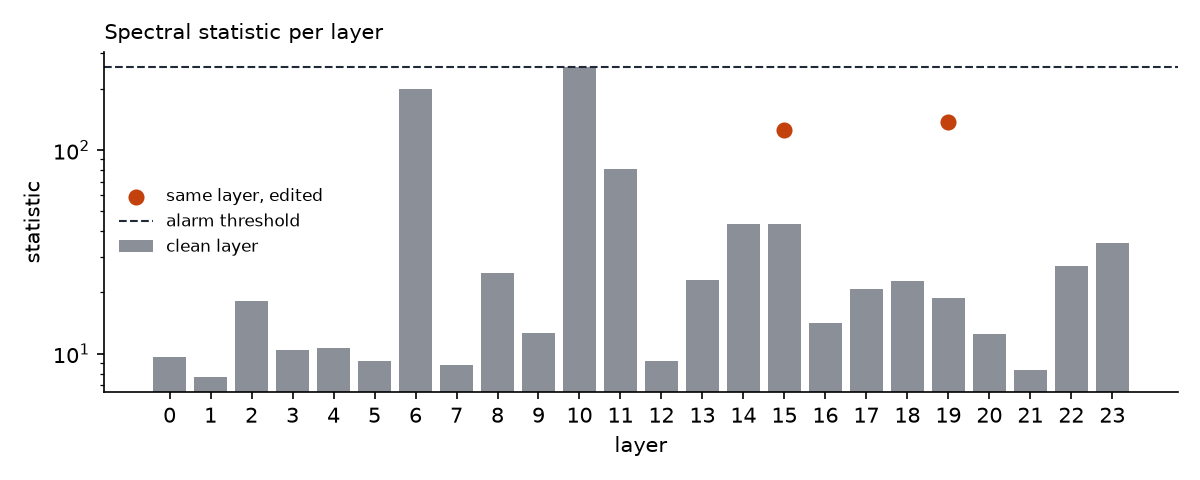
\includegraphics[width=0.92\textwidth]{fig_screen.png}
\caption{Spectral statistic $T$ of every layer of the clean model (bars) and of the two layers
changed by the published edit (dots). The dashed line is the alarm threshold, 255.9. The vertical
axis is logarithmic.}
\label{fig:screen}
\end{figure}

\section{Interpretation and limits}

Often the weights alone will tell you where such an edit falls. They do not signal that a
checkpoint has been edited: the pattern this detector looks for is already present in clean layers,
so there is no threshold on its statistic that can tell them apart. An edit half the size is rarely
found (1 of 28 localised), and one aligned with a direction already used by the layer is found
unreliably.

This is one model, two detectors and one published edit in two layers. The synthetic edits all
come from one family, and the threshold needs known-clean weights to calibrate. I did not test the
article's other two edits (one spread over 30 matrices, one in an attention head, which these
detectors do not look at), or whether ordinary fine-tuning raises alarms. The localisation result
missed its bar (0.77 against 0.80), so I report it as inconclusive. The Swedish prose and English
maths passages are not matched, so the loss result does not show the edit is specific to Swedish.
Random edits also cost more on the Swedish set.

\section{Recommendation and next experiment}

\begin{itemize}
\item Do not rely on weight inspection to vet third-party weights. Verify the hash against a
trusted source, and run a Swedish behavioural check on every checkpoint or edit adopted.
\item Treat edits found by English feedback as untested in Swedish. The one published example has a
measurable Swedish cost that its English evaluation never saw.
\item I would keep watching the article's approach without building on it yet. Its language-model
result is a fix for one particular failure, found by a 20-hour feedback loop, with no comparison to
standard steering.
\end{itemize}

The most informative next experiment would be to build an edit that intentionally lowers Swedish
quality but not English, on matched parallel text, at several sizes. If Swedish can be damaged by
an edit smaller than these detectors can localise (they localised 1 of 28 at 5\%), they offer no
defence and a stronger weight statistic would be needed. This will give more indication that the
model owner can intentionally edit the weights to hinder development for a specific area of
research. It would be less evident than a restriction that can be done during training, where the
model is trained to deny work along a subject matter.

\end{document}
